
\begin{figure}[!t]
\centering
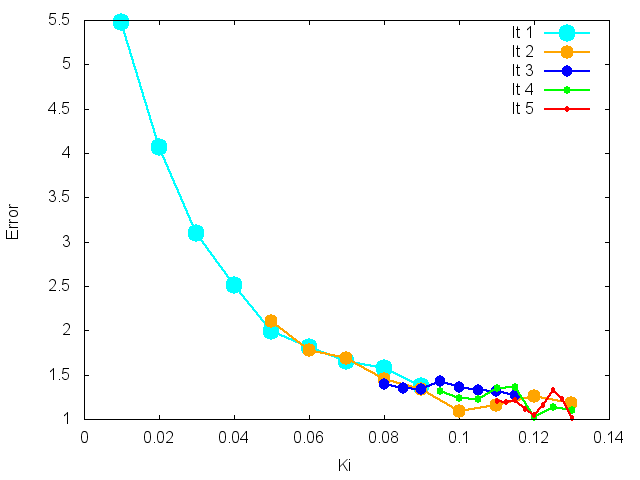
\includegraphics[width=3in]{./figures/Results/ki.png}

\caption{Error based on different $K$ values with iteration number $It$}
\label{Ki}
\end{figure}




\begin{figure}[!t]
\centering
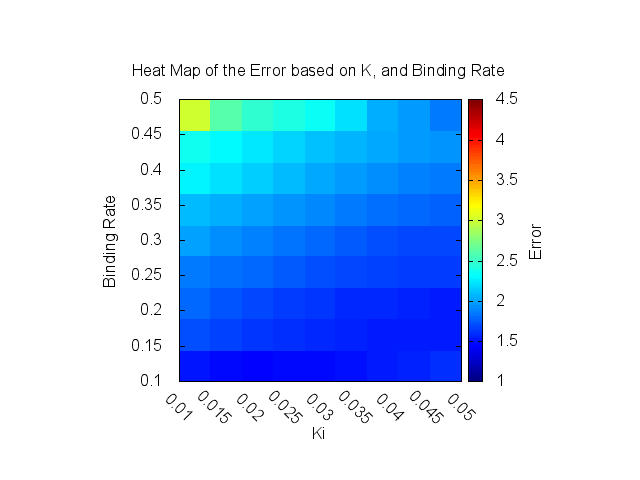
\includegraphics[width=3in]{./figures/Results/KiB1.png}

\caption{The heat map of error between $K$ and VEGF binding coefficient/rate ($\beta$) determined from the first round sweep.}
\label{KiB1}
\end{figure}



\begin{figure}[!t]
\centering
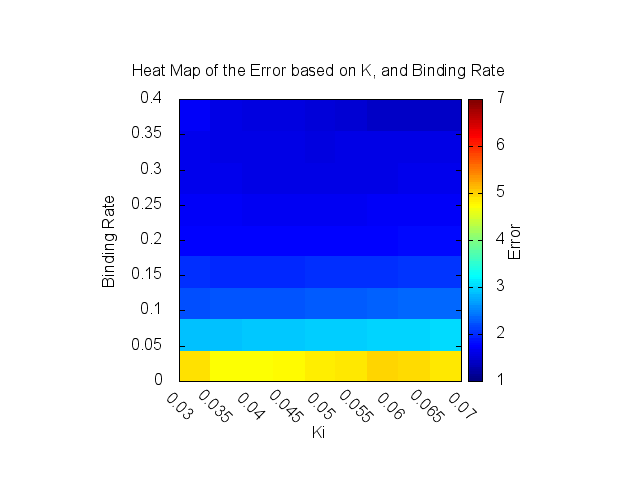
\includegraphics[width=3in]{./figures/Results/KiB2.png}

\caption{The heat map of error between $K$ and VEGF binding coefficient/rate ($\beta$) determined from the second round sweep.}
\label{KiB2}
\end{figure}


\begin{figure}[!t]
\centering
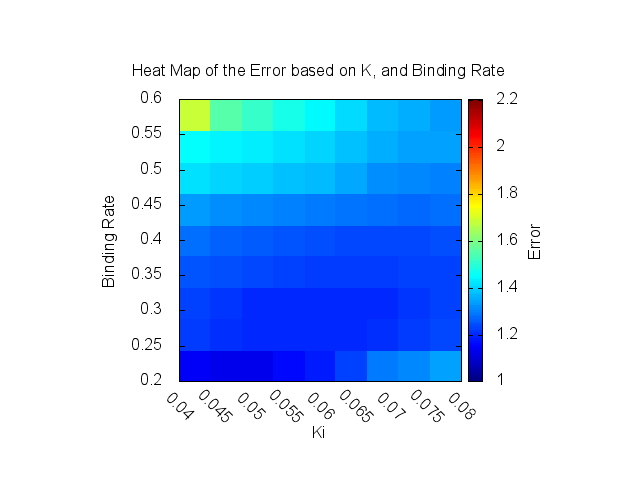
\includegraphics[width=3in]{./figures/Results/KiB3.png}

\caption{The heat map of error between $K$ and VEGF binding coefficient/rate ($\beta$) from the third round sweep.}
\label{KiB3}
\end{figure}


Initially the method was applied to a single parameter, $K$. Figure \ref{Ki} shows the error values for five sweep iterations over $K$. In each iteration, a parameter sweep for each patch size was performed. In this run, the values of VEGF secretion rate $\mu _{V}$ and VEGF binding rate $\beta$ were set to 0.09 pg/ml and 1.0, respectively. In iteration 1 ($It1$) the parameters were swept from 0.1 to 0.9, then the best value was chosen to determine the sweeping range for iteration 2 ($It2$). Over repeated sweeps the range of possible valid values for $K$ was greatly reduced. After five iterations of sweep processes, the best $K$ value obtained was 0.13 and the associated error was 1.01. This search considered many potential solutions and all but one were rejected as sub-optimal.

Figure \ref{KiB1} shows the error heat map of the first sweep iteration ($It1$) over two parameters ($K$ and $\beta$). For this run, the VEGF secretion rate $\mu _{V}$ was set to 0.078 pg/ml/hour. As shown, the error is lowest when the VEGF binding rate ($\beta$) is less than 0.3 and the $K$ value is greater than 0.03. Figure \ref{KiB2} shows the second sweep ($It2$), which has adjusted sweeping ranges for $K$ and $\beta$. Successive iterations refine the parameter values, as shown through reduced error in Figure \ref{KiB3}, which shows the third sweep ($It3$). The same sweeping processes was also performed between ($\mu _{V}$ and $K$) and ($\mu _{V}$ and $\beta$) (data not shown).

To show how the concentration of VEGF changes over time in the simulation, VEGF expression levels were calculated at various time intervals (4, 24, 30, 48, 54, 72 h). Figure \ref{In-Vitro_Data} shows the data from \textit{in vitro} and Figure \ref{AfterOpt} the \textit{in silico} model, $K$, $\mu _{V}$, and $\beta$ are set to 0.2, 0.07874 and 0.899, respectively, which were determined from a near-optimal solution discovered by the search method. The error associated with these results is 0.925. %as shown in the results obtained from the \textit{in vitro} experiments and the \textit{in silico} model outputs in Figure \ref{In-Vitro_Data}, and Figure \ref{AfterOpt}, respectively,
As shown in figure \ref{In-Vitro_Data} and \ref{AfterOpt}, in both \textit{in silico} and \textit{in vitro}, RPE cells in the smaller patches expressed higher levels of VEGF per cell. This indicates that these cells function to maintain a consistent level of VEGF within their local microenvironment. Cells in smaller patches respond by expressing higher amounts of VEGF because the VEGF expression levels are dominated by cell-environment interactions. In contrast, larger patches maintain lower basal levels of VEGF because cell-cell auto-inhibitory regulation dominates.

Now the parameters $K$, $\mu_V$ and $\beta$ have been determined, we replace the variables with their values in Equation~\ref{VEGF_autoregulation} and set the mass $M$ to that of a single cell ($M = 25.95 pg$) resulting in the VEGF autoregulatory function for RPE cells being:

\begin{equation}
 \frac{d V}{d t}= 0.07874 \times \frac{0.2}{ 0.899 V+0.2} \times 25.95
 \label{VEGF_final}
 \end{equation}

This function is plotted in Figure~\ref{finalGraph}.

\begin{figure}[!t]
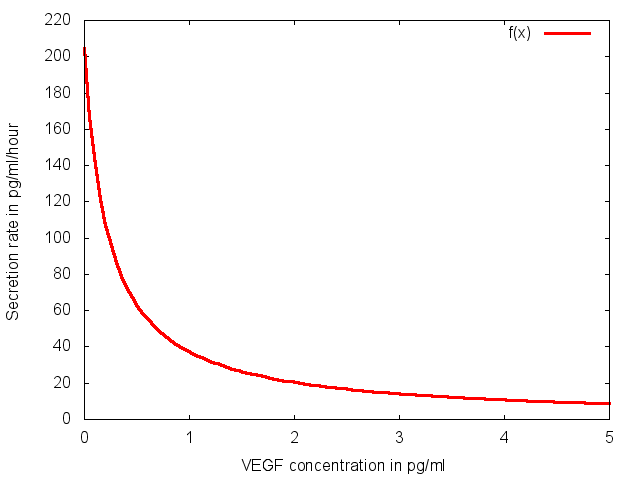
\includegraphics[width=.8\linewidth]{./figures/Results/Final_Result.png}
   \caption{The VEGF autoregulatory function of RPE cells showing how the secretion rate of VEGF is down regulated as a function of the VEGF in the microenvironment.}
   \label{finalGraph}
   \end{figure}

  \begin{figure}[!t]
  \centering


 \begin{subfigure}{.5\textwidth}
   \centering
   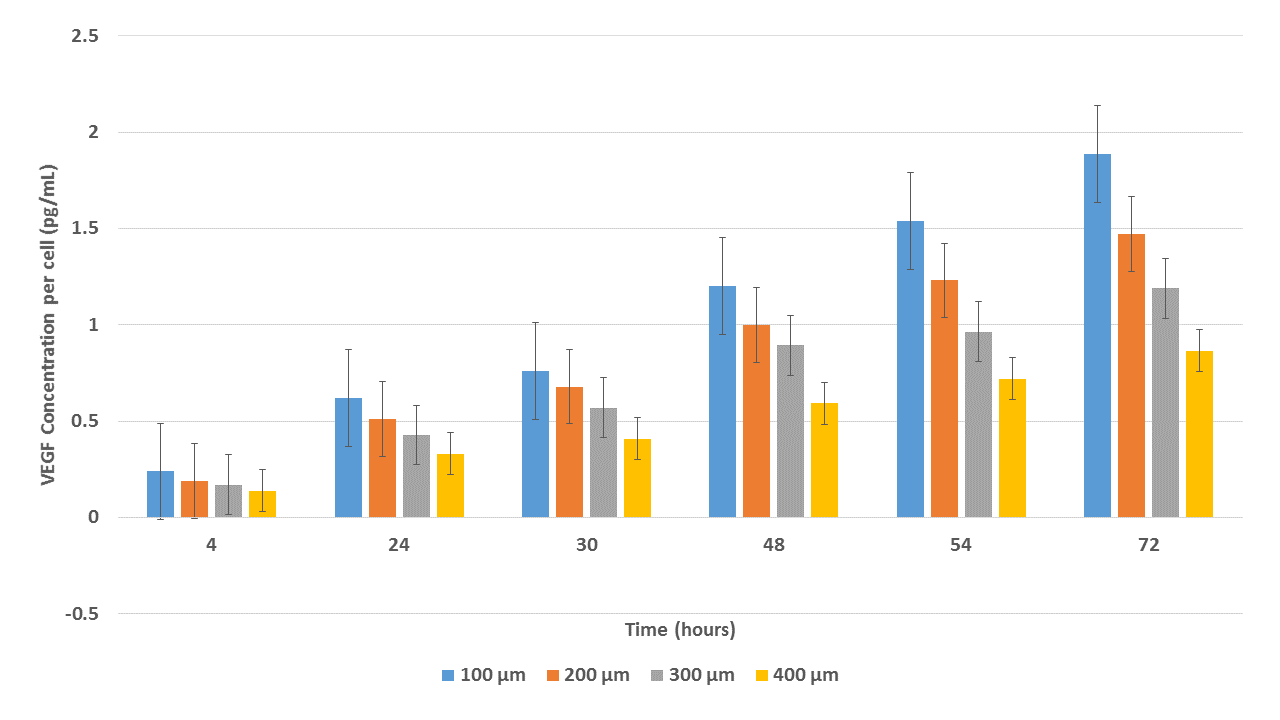
\includegraphics[width=.8\linewidth]{./figures/Results/In-Vitro.png}
   \caption{Time course of VEGF expression per cell measured at 4, 24, 30, 48, and 72 h (data from the \textit{in vitro} work \cite{qanitabaker:Vargis2014Effect} ).}
   \label{In-Vitro_Data}
 \end{subfigure}%


  \begin{subfigure}{.5\textwidth}
    \centering
    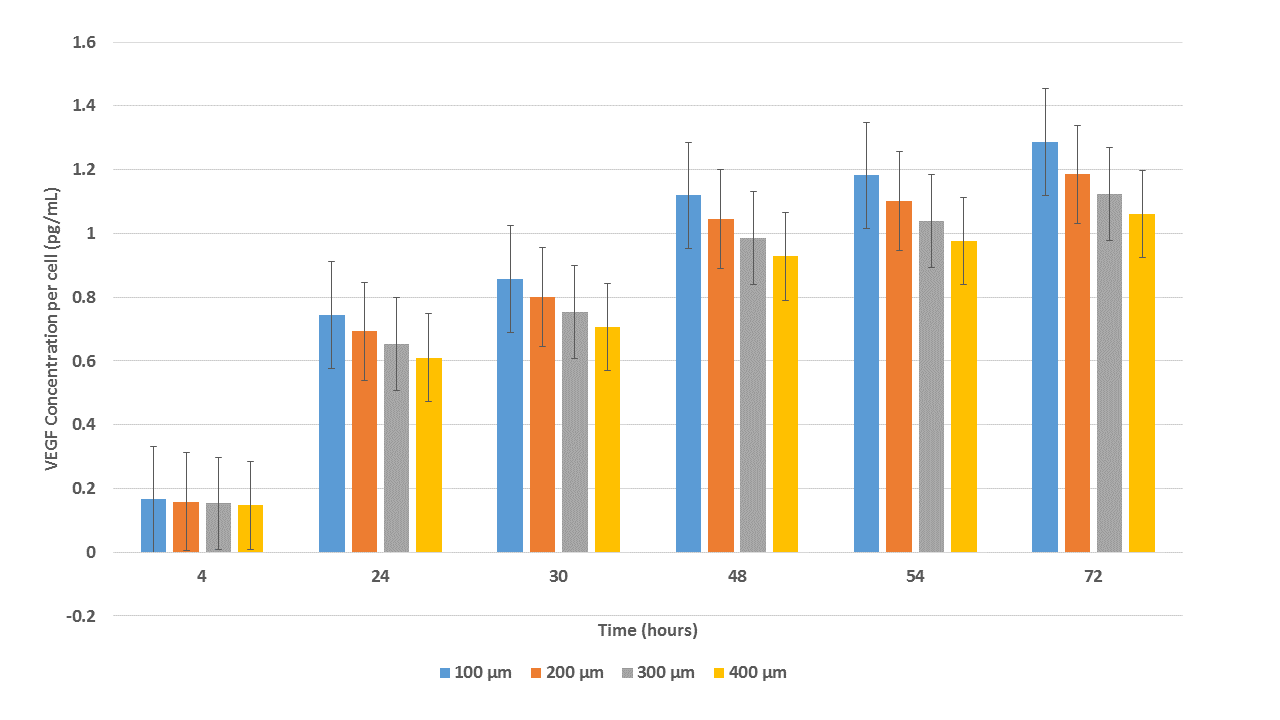
\includegraphics[width=.8\linewidth]{./figures/Results/After.png}
    \caption{Time course of VEGF expression per cell measured at 4, 24, 30, 48, and 72 h (data from the \textit{in silico} model after optimization).}
    \label{AfterOpt}
  \end{subfigure}%

  \end{figure}
